\documentclass{beamer}
\usepackage[utf8]{inputenc}
\usetheme{Ilmenau}
\usepackage[frenchb]{babel}    % le documents est en français
\usepackage{amsmath}           % un packages mathématiques
\usepackage{xcolor}            % pour définir plus de couleurs 
\usepackage{graphicx}          % pour insérer des figures
		
\usepackage{Slides_08092010}

  \title{Amélioration de la réactivité des réseaux pair à pair pour les MMOGs}
  \author{Xavier Joudiou,\\\tiny{Encadré par: S.Legtchenko \& S.Monnet}}\institute{Université Paris VI, Master SAR}
 % \logo{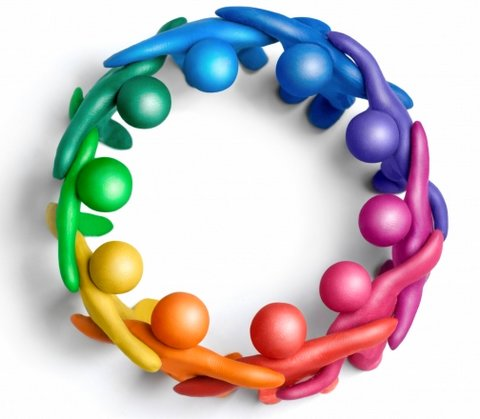
\includegraphics[scale=0.5]{./Ressources/Images/P2P.png}}
  \date{8 Septembre 2010}

  \begin{document}

  \begin{frame}
  \maketitle
  \end{frame}


  \begin{frame}
  \tableofcontents
  \end{frame}

  \section{Introduction}
  \begin{frame}
	Nous présenter les concepts nécessaires à une bonne compréhension des solutions qu'il nous a été possible d'implémenter.
  \end{frame}
	
  \section{État de l'art}
  \begin{frame}
	Présentation des différents solutions sur lesquels, nos solutions s'appuient.
	\begin{itemize}
		\item Solipsis
		\item Étude des traces des joueurs de MMOG
		\item Blue Banana
	\end{itemize}
  \end{frame}

  \subsection{Solipsis}

  \begin{frame}
 Solipsis est un travail qui propose un monde virtuel entièrement décentralisé et scalable. Un overlay qui est caractérisé par une forte malléabilité applicative, sert de support au monde virtuel.

  \end{frame}

  \begin{frame}
	Solipsis introduit plusieurs propriétés:
	\begin{itemize}
                \item \textit{Local Awareness:}\\
                Une entité doit être connectée avec tous ses plus proches voisins, elle peut de connaître des entités en dehors de son environnement virtuel local. Toute entité située à l'intérieur doit partie des voisins de l'entité.
                \item \textit{Global Connectivity:}\\
                Toute entité virtuelle doit se trouver à l'intérieur de l'enveloppe convexe contenant l'ensemble de ses voisins logiques. \\
	\end{itemize}
  \end{frame}

  \subsection{Les traces}
  \begin{frame}
	Des études des traces des joueurs de MMOG, ont permis de détecter différents habitudes des joueurs:
	\begin{itemize}
		\item Zones dense 
		\item Mouvements erratiques dans les zones denses
		\item Mouvements rectiligne et rapide entre les zones denses
	\end{itemize}
  \end{frame}

  \subsection{BlueBanana}
  \begin{frame}
	 Trois états, pour un avatar, ont été introduits:
        \begin{itemize}
                \item \textbf{H}(alted): l'avatar est immobile.
                \item \textbf{T}(ravelling): l'avatar se déplace rapidement sur la carte et il a une trajectoire droite.
                \item \textbf{E}(xploring): l'avatar est en train d'explorer une zone, sa trajectoire est confuse et sa vitesse est lente.
        \end{itemize}
  \end{frame}

  \begin{frame}
	Mise en place d'un mécanisme d'anticipation des mouvements des avatars.
	\begin{columns}
	  \begin{column}{5cm}
		\begin{itemize}
		  \item bli
		  \item blo
		  \item bla
		\end{itemize}
	  \end{column}
	\begin{column}{5cm}
	\begin{figure}
        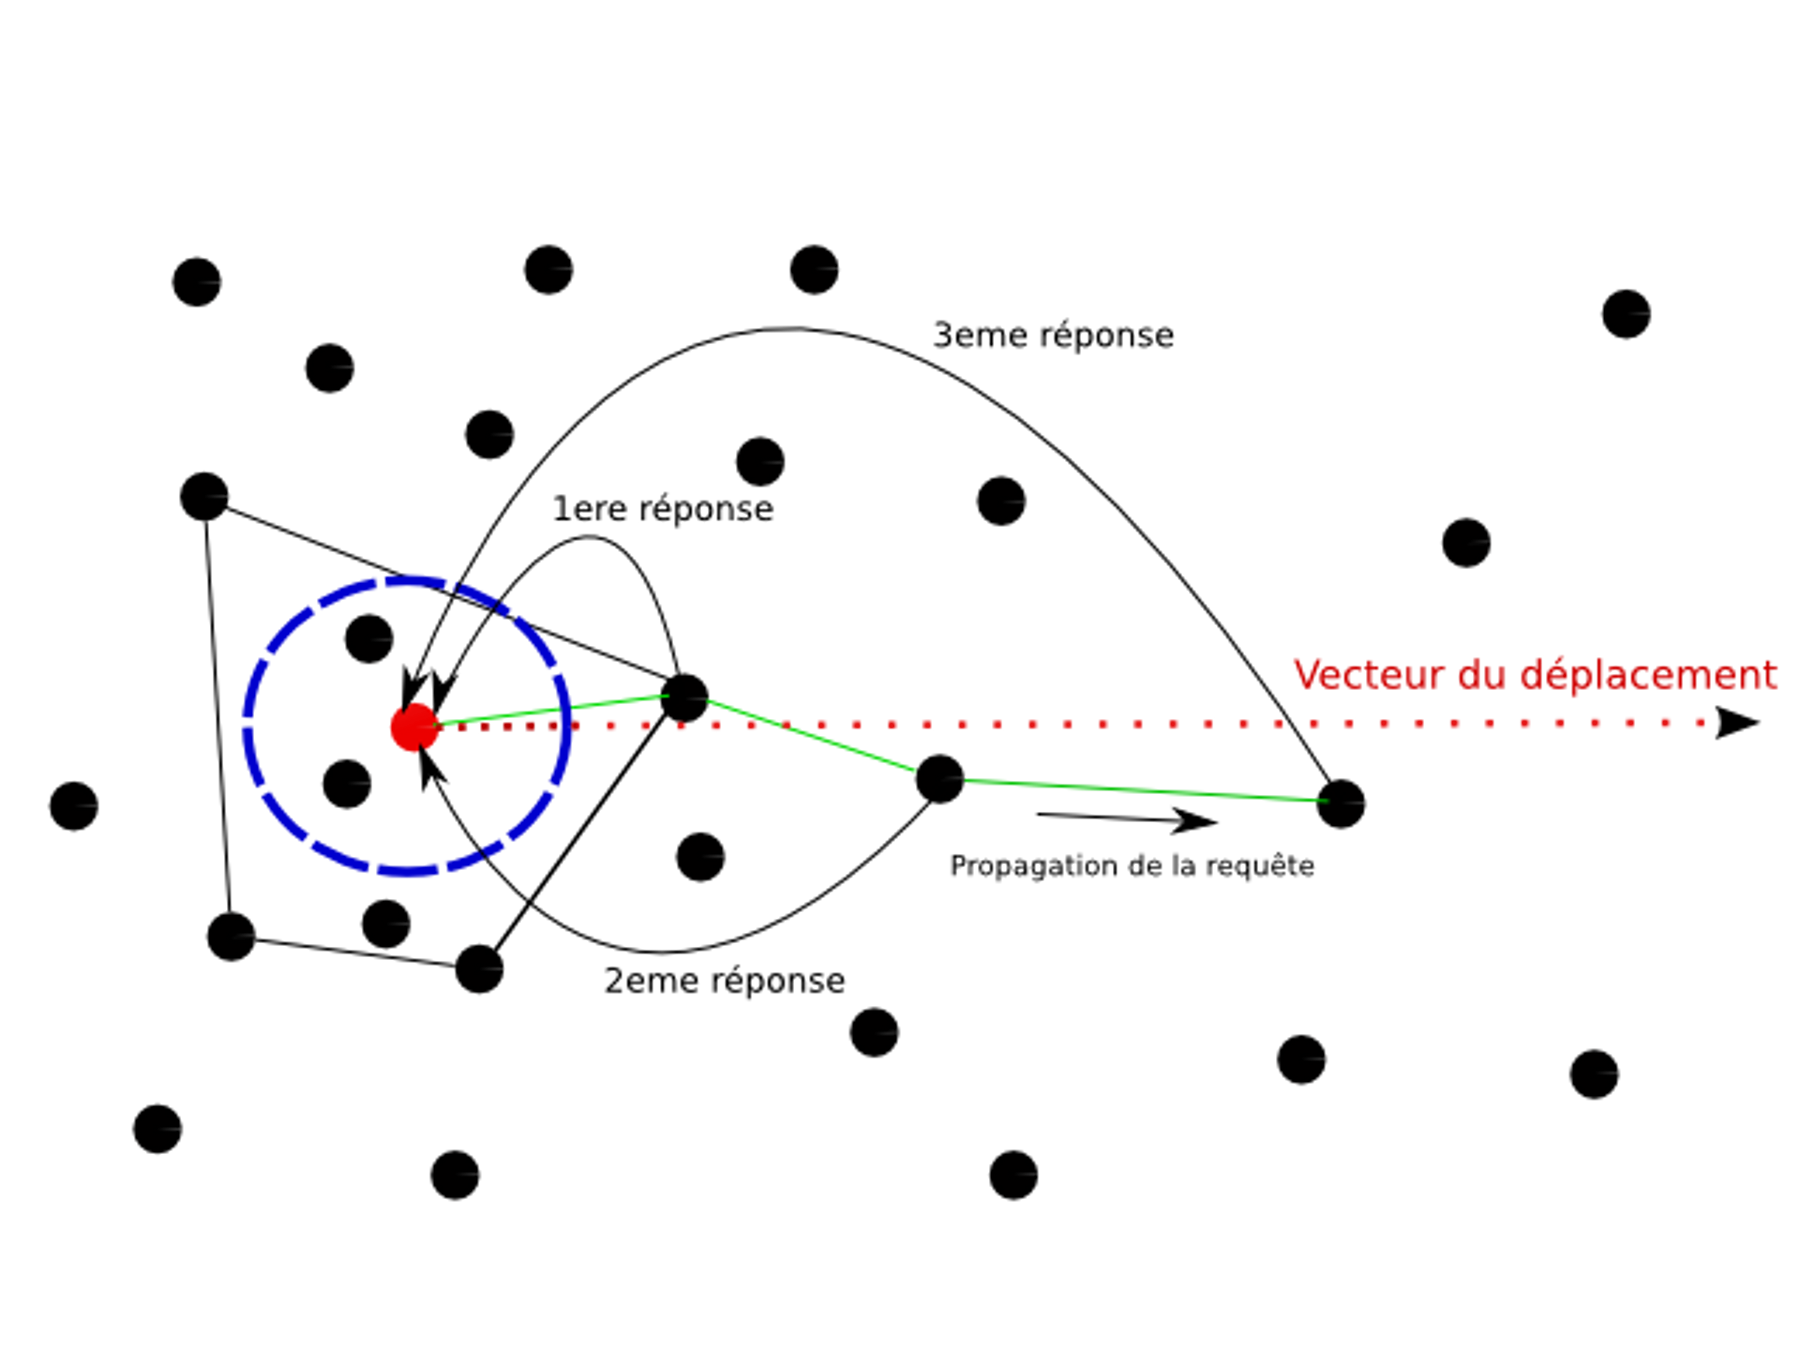
\includegraphics[scale=0.3]{./Ressources/Images/propagation_algo.png}\\
        \label{Propa_Algo}
        \end{figure}
	\end{column}
	\end{columns}

  \end{frame}

  \section{Les améliorations}
  \begin{frame}
	Durant le stage, plusieurs solutions ont été implémentées:
	\begin{itemize}
		\pause\item Le cache pour les zones dense
		\pause\item Le préchargement amélioré des données
	\end{itemize}
  \end{frame}

  \begin{frame}
	Les différentes métriques utilisées pour analyser les tests sont:
	\begin{itemize}
		\item Nombre de messages
		\item Cohérence de la topologie
		\item Cache Hit et Miss (pour le cache)
	\end{itemize}
  \end{frame}

  \section{Le cache pour les zones denses}
  \begin{frame}
	Les explications sur le cache se décomposeront comme cela:
	\begin{itemize}
		\item Explications sur le cache des zones denses
		\item Les résultats 
		\item Conclusion sur la cache
	\end{itemize}
  \end{frame}
  
  \subsection{Explications du cache pour les zones denses}
  \begin{frame}
	On explique comment marche le cache
  \end{frame}
  
  \subsection{Résultats pour le cache}
  \begin{frame}
	Résultats pour le cache des zones denses
  \end{frame}

  \begin{frame}
	Résultats pour le cache des zones denses suite
  \end{frame}
	
  \subsection{Conclusion sur le cache des zones denses}
  \begin{frame}
	Ca marche pas trop mal non?
  \end{frame}



  \section{Le préchargement amélioré des données}
  \begin{frame}
	Les explications sur le préchargement amélioré se décomposeront comme cela:
	\begin{itemize}
		\item Explications sur le préchargement amélioré
		\item Les résultats 
		\item Conclusion sur la préchargement
	\end{itemize}
  \end{frame}

  \subsection{Explications du préchargement amélioré}
  \begin{frame}
	On explique comment marche le préchargement
  \end{frame}

  \begin{frame}
	Fin explications préchargement amélioré
  \end{frame}
	
  \subsection{Résultats pour le préchargement amélioré}
  \begin{frame}
	Résultats préchargement amélioré
  \end{frame}
	
  \begin{frame}
	Résultats préchargement amélioré suite
  \end{frame}

  \subsection{Conclusion sur le préchargement amélioré}
  \begin{frame}
	Ca marche pas trop mal non?
  \end{frame}
	
  
  \section{Conclusion}
  \begin{frame}
  \end{frame}
  
  \end{document}
